\documentclass{article}
\usepackage[utf8]{inputenc}
\usepackage{graphicx}
\usepackage{booktabs}
\usepackage{float}
\graphicspath{ {./metrics/fold_0/} }
\graphicspath{ {./metrics/fold_1/} }
\title{Results: bert-base-uncased-baseline-plg-[cls]-lr-[0.00005|0.00001|0.000001]-folds-[2]}
\author{Nadia Sheikh}
\date{2022-07-27}
\begin{document}
\maketitle
\section{Configurations}
\subsection{Run Configuration}
\begin{tabular}{ll}
\toprule
{} &                                                  0 \\
\midrule
experiment\_identifier &                          llm-baseline-[bert|sbert] \\
run\_identifier        &  bert-base-uncased-baseline-plg-[cls]-lr-[0.000... \\
config\_file\_path      &  /tmp/71354.1.all.q/ctre/cnc-task-3/runs/config... \\
\bottomrule
\end{tabular}

\subsection{Data Configuration}
\begin{tabular}{ll}
\toprule
{} &                                                  0 \\
\midrule
data\_utility\_cls        &                                      cnc\_utilities \\
dataset\_cls             &                                   CNCTask3aDataset \\
nos\_of\_folds            &                                                  2 \\
trn\_data\_path           &  /cnc-task-3/data/csv-gold-standard/training-data/ \\
tst\_data\_path           &  /home/nadia/Documents/CLaC-Lab/ctre/cnc-task-3... \\
base\_output\_folder\_path &                           /cnc-task-3/experiments/ \\
config\_file\_path        &  /tmp/71354.1.all.q/ctre/cnc-task-3/runs/config... \\
\bottomrule
\end{tabular}

\subsection{Preprocessing Configuration}
\begin{tabular}{ll}
\toprule
{} &                                                  0 \\
\midrule
collate\_fn\_name   &                                       LLMCollateFn \\
llm\_name          &                                  bert-base-uncased \\
connl\_folder\_path &  /home/nadia/Documents/CLaC-Lab/ctre/cnc-task-3... \\
max\_nos\_tokens    &                                                 84 \\
token\_sep         &                                               True \\
config\_file\_path  &  /tmp/71354.1.all.q/ctre/cnc-task-3/runs/config... \\
\bottomrule
\end{tabular}

\section{Hyperparameters}
\subsection{hparam\_config\_id\_0}
\begin{tabular}{ll}
\toprule
{} &                   0 \\
\midrule
loss\_function                    &  cross-entropy-loss \\
learning\_rate                    &             0.00005 \\
batch\_size                       &                   1 \\
optimizer                        &                adam \\
llm                              &   bert-base-uncased \\
llm\_hidden\_dropout\_prob          &                 0.1 \\
llm\_attention\_probs\_dropout\_prob &                 0.1 \\
pooling                          &                 cls \\
classes                          &                   2 \\
max\_epochs                       &                  10 \\
\bottomrule
\end{tabular}

\subsection{hparam\_config\_id\_1}
\begin{tabular}{ll}
\toprule
{} &                   0 \\
\midrule
loss\_function                    &  cross-entropy-loss \\
learning\_rate                    &             0.00001 \\
batch\_size                       &                   1 \\
optimizer                        &                adam \\
llm                              &   bert-base-uncased \\
llm\_hidden\_dropout\_prob          &                 0.1 \\
llm\_attention\_probs\_dropout\_prob &                 0.1 \\
pooling                          &                 cls \\
classes                          &                   2 \\
max\_epochs                       &                  10 \\
\bottomrule
\end{tabular}

\subsection{hparam\_config\_id\_2}
\begin{tabular}{ll}
\toprule
{} &                   0 \\
\midrule
loss\_function                    &  cross-entropy-loss \\
learning\_rate                    &            0.000005 \\
batch\_size                       &                   1 \\
optimizer                        &                adam \\
llm                              &   bert-base-uncased \\
llm\_hidden\_dropout\_prob          &                 0.1 \\
llm\_attention\_probs\_dropout\_prob &                 0.1 \\
pooling                          &                 cls \\
classes                          &                   2 \\
max\_epochs                       &                  10 \\
\bottomrule
\end{tabular}

\section{fold\_0}
\subsection{train\_loss}
\begin{tabular}{lrrrrrrrrrr}
\toprule
{} &   ep 0 &   ep 1 &   ep 2 &   ep 3 &   ep 4 &   ep 5 &   ep 6 &   ep 7 &   ep 8 &   ep 9 \\
\midrule
hp\_0 &  0.653 &  0.561 &  0.429 &  0.469 &  0.557 &  0.697 &  0.702 &  0.699 &  0.697 &  0.695 \\
hp\_1 &  0.581 &  0.261 &  0.057 &  0.011 &  0.001 &  0.025 &  0.027 &  0.001 &  0.000 &  0.000 \\
hp\_2 &  0.602 &  0.339 &  0.085 &  0.009 &  0.001 &  0.000 &  0.000 &  0.000 &  0.000 &  0.000 \\
\bottomrule
\end{tabular}

\begin{figure}[H]
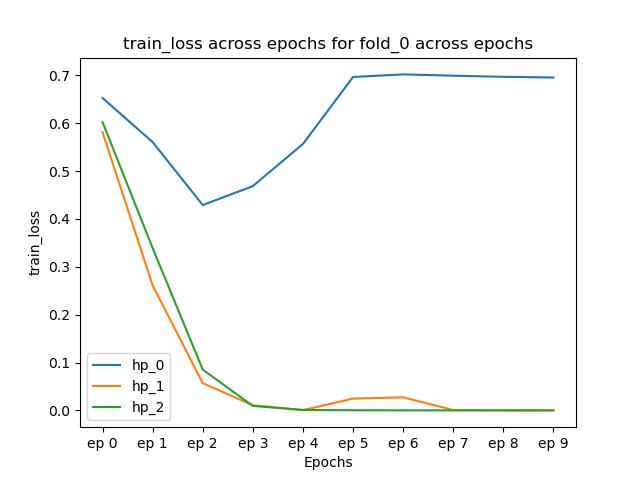
\includegraphics[scale = 0.75]{fold_0/train_loss}
\end{figure}
\subsection{test\_loss}
\begin{tabular}{lrrrrrrrrrr}
\toprule
{} &   ep 0 &   ep 1 &   ep 2 &   ep 3 &   ep 4 &   ep 5 &   ep 6 &   ep 7 &   ep 8 &   ep 9 \\
\midrule
hp\_0 &  0.706 &  0.665 &  0.637 &  0.628 &  0.690 &  0.689 &  0.697 &  0.688 &  0.688 &  0.689 \\
hp\_1 &  0.505 &  0.501 &  0.737 &  0.896 &  1.190 &  0.916 &  0.845 &  1.143 &  1.231 &  1.308 \\
hp\_2 &  0.536 &  0.489 &  0.613 &  0.837 &  0.954 &  1.065 &  1.175 &  1.285 &  1.395 &  1.504 \\
\bottomrule
\end{tabular}

\begin{figure}[H]
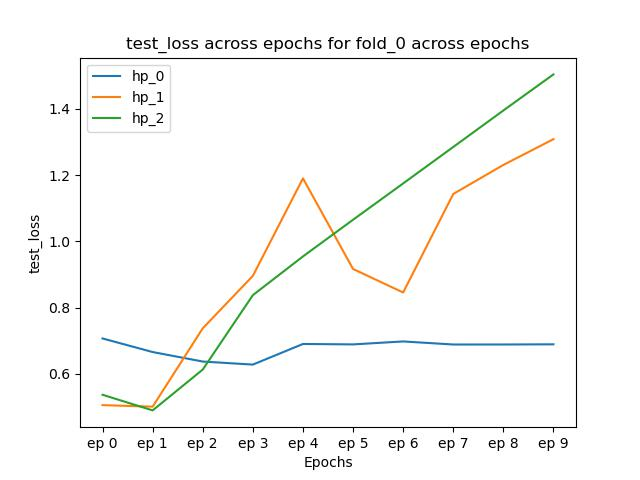
\includegraphics[scale = 0.75]{fold_0/test_loss}
\end{figure}
\subsection{accuracy\_score}
\begin{tabular}{lrrrrrrrrrr}
\toprule
{} &  ep 0 &   ep 1 &   ep 2 &   ep 3 &   ep 4 &   ep 5 &   ep 6 &   ep 7 &   ep 8 &   ep 9 \\
\midrule
hp\_0 &  0.55 &  0.582 &  0.670 &  0.660 &  0.550 &  0.550 &  0.550 &  0.550 &  0.550 &  0.550 \\
hp\_1 &  0.75 &  0.786 &  0.780 &  0.797 &  0.793 &  0.786 &  0.795 &  0.797 &  0.799 &  0.800 \\
hp\_2 &  0.73 &  0.768 &  0.794 &  0.796 &  0.804 &  0.805 &  0.807 &  0.809 &  0.808 &  0.808 \\
\bottomrule
\end{tabular}

\begin{figure}[H]
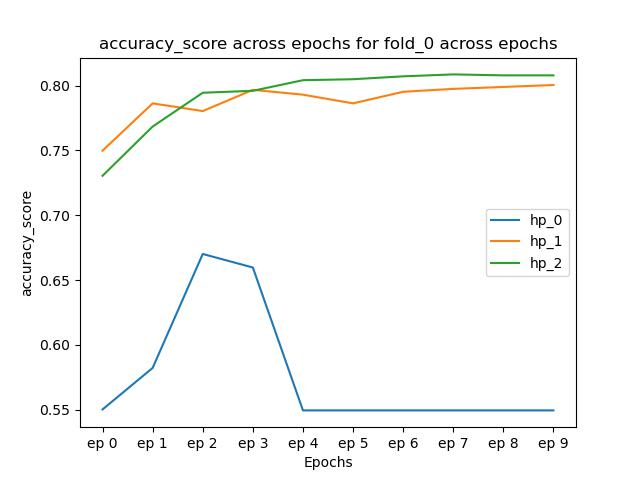
\includegraphics[scale = 0.75]{fold_0/accuracy_score}
\end{figure}
\subsection{f1\_score}
\begin{tabular}{lrrrrrrrrrr}
\toprule
{} &   ep 0 &   ep 1 &   ep 2 &   ep 3 &   ep 4 &   ep 5 &   ep 6 &   ep 7 &   ep 8 &   ep 9 \\
\midrule
hp\_0 &  0.710 &  0.722 &  0.760 &  0.758 &  0.709 &  0.709 &  0.709 &  0.709 &  0.709 &  0.709 \\
hp\_1 &  0.799 &  0.813 &  0.781 &  0.813 &  0.798 &  0.817 &  0.813 &  0.825 &  0.825 &  0.825 \\
hp\_2 &  0.786 &  0.806 &  0.814 &  0.811 &  0.821 &  0.822 &  0.824 &  0.825 &  0.824 &  0.824 \\
\bottomrule
\end{tabular}

\begin{figure}[H]
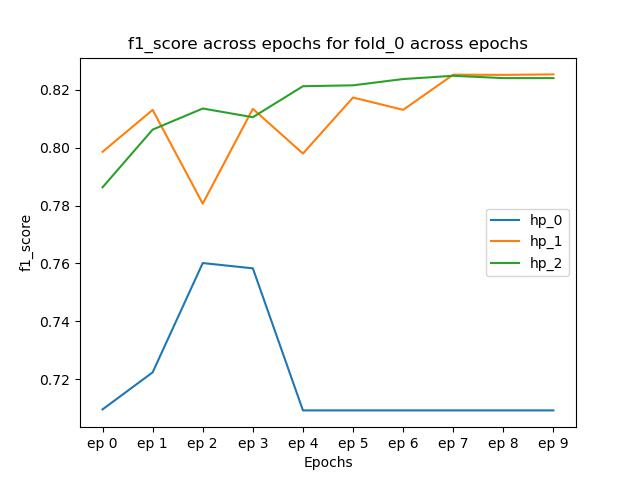
\includegraphics[scale = 0.75]{fold_0/f1_score}
\end{figure}
\subsection{precision\_score}
\begin{tabular}{lrrrrrrrrrr}
\toprule
{} &   ep 0 &   ep 1 &   ep 2 &   ep 3 &   ep 4 &   ep 5 &   ep 6 &   ep 7 &  ep 8 &   ep 9 \\
\midrule
hp\_0 &  0.550 &  0.569 &  0.633 &  0.622 &  0.550 &  0.550 &  0.550 &  0.550 &  0.55 &  0.550 \\
hp\_1 &  0.716 &  0.783 &  0.865 &  0.821 &  0.861 &  0.771 &  0.816 &  0.785 &  0.79 &  0.795 \\
hp\_2 &  0.697 &  0.746 &  0.811 &  0.828 &  0.824 &  0.826 &  0.828 &  0.830 &  0.83 &  0.830 \\
\bottomrule
\end{tabular}

\begin{figure}[H]
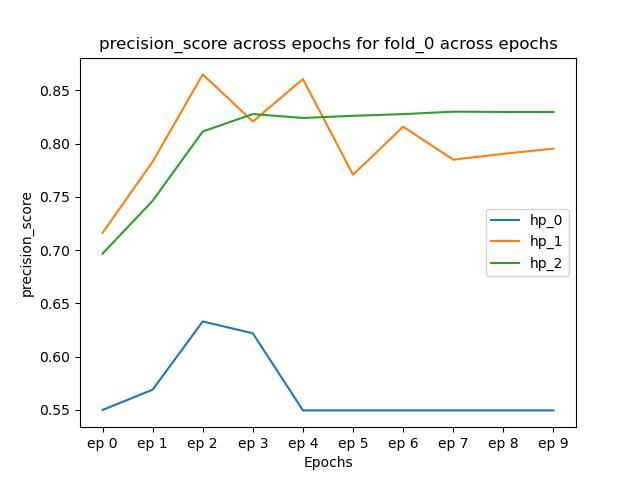
\includegraphics[scale = 0.75]{fold_0/precision_score}
\end{figure}
\subsection{matthews\_corrcoef}
\begin{tabular}{lrrrrrrrrrr}
\toprule
{} &   ep 0 &   ep 1 &   ep 2 &   ep 3 &   ep 4 &   ep 5 &   ep 6 &   ep 7 &   ep 8 &   ep 9 \\
\midrule
hp\_0 &  0.030 &  0.181 &  0.365 &  0.358 &  0.000 &  0.000 &  0.000 &  0.000 &  0.000 &  0.000 \\
hp\_1 &  0.503 &  0.567 &  0.576 &  0.590 &  0.595 &  0.568 &  0.587 &  0.590 &  0.593 &  0.596 \\
hp\_2 &  0.465 &  0.534 &  0.585 &  0.590 &  0.605 &  0.606 &  0.611 &  0.614 &  0.613 &  0.613 \\
\bottomrule
\end{tabular}

\begin{figure}[H]
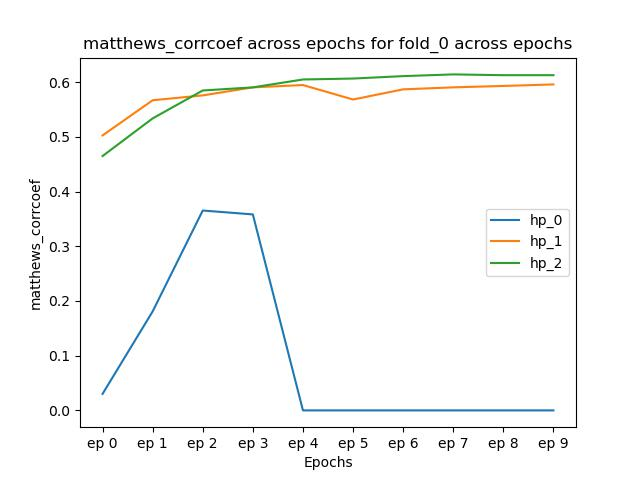
\includegraphics[scale = 0.75]{fold_0/matthews_corrcoef}
\end{figure}
\subsection{recall\_score}
\begin{tabular}{lrrrrrrrrrr}
\toprule
{} &   ep 0 &   ep 1 &   ep 2 &   ep 3 &   ep 4 &   ep 5 &  ep 6 &  ep 7 &   ep 8 &   ep 9 \\
\midrule
hp\_0 &  1.000 &  0.989 &  0.951 &  0.972 &  1.000 &  1.000 &  1.00 &  1.00 &  1.000 &  1.000 \\
hp\_1 &  0.902 &  0.846 &  0.711 &  0.806 &  0.744 &  0.870 &  0.81 &  0.87 &  0.863 &  0.858 \\
hp\_2 &  0.902 &  0.877 &  0.816 &  0.794 &  0.818 &  0.817 &  0.82 &  0.82 &  0.818 &  0.818 \\
\bottomrule
\end{tabular}

\begin{figure}[H]
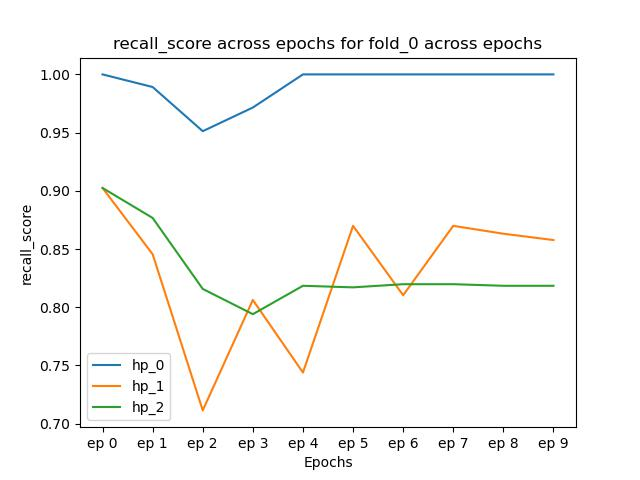
\includegraphics[scale = 0.75]{fold_0/recall_score}
\end{figure}
\section{fold\_1}
\subsection{train\_loss}
\begin{tabular}{lrrrrrrrrrr}
\toprule
{} &   ep 0 &   ep 1 &   ep 2 &   ep 3 &   ep 4 &   ep 5 &   ep 6 &   ep 7 &   ep 8 &   ep 9 \\
\midrule
hp\_0 &  0.715 &  0.699 &  0.695 &  0.694 &  0.692 &  0.691 &  0.692 &  0.691 &  0.691 &  0.691 \\
hp\_1 &  0.585 &  0.242 &  0.061 &  0.026 &  0.023 &  0.016 &  0.011 &  0.009 &  0.002 &  0.036 \\
hp\_2 &  0.637 &  0.359 &  0.058 &  0.019 &  0.008 &  0.018 &  0.002 &  0.000 &  0.000 &  0.000 \\
\bottomrule
\end{tabular}

\begin{figure}[H]
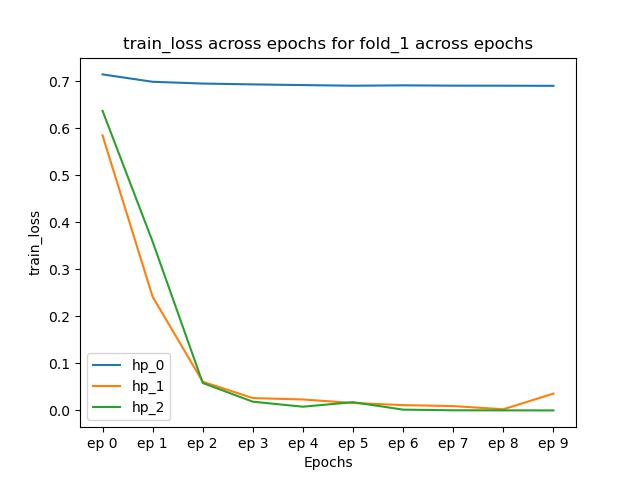
\includegraphics[scale = 0.75]{fold_1/train_loss}
\end{figure}
\subsection{test\_loss}
\begin{tabular}{lrrrrrrrrrr}
\toprule
{} &   ep 0 &   ep 1 &   ep 2 &   ep 3 &   ep 4 &   ep 5 &   ep 6 &   ep 7 &   ep 8 &   ep 9 \\
\midrule
hp\_0 &  0.691 &  0.689 &  0.689 &  0.689 &  0.689 &  0.689 &  0.689 &  0.689 &  0.689 &  0.689 \\
hp\_1 &  0.436 &  0.591 &  0.744 &  1.047 &  1.135 &  1.153 &  1.273 &  1.070 &  1.301 &  1.038 \\
hp\_2 &  0.522 &  0.489 &  0.704 &  0.861 &  1.989 &  0.889 &  1.020 &  1.102 &  1.161 &  1.236 \\
\bottomrule
\end{tabular}

\begin{figure}[H]
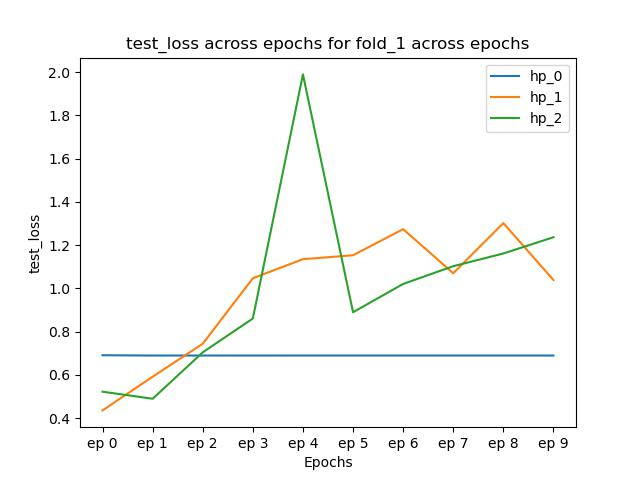
\includegraphics[scale = 0.75]{fold_1/test_loss}
\end{figure}
\subsection{accuracy\_score}
\begin{tabular}{lrrrrrrrrrr}
\toprule
{} &   ep 0 &   ep 1 &   ep 2 &   ep 3 &   ep 4 &   ep 5 &   ep 6 &   ep 7 &   ep 8 &   ep 9 \\
\midrule
hp\_0 &  0.544 &  0.544 &  0.544 &  0.544 &  0.544 &  0.544 &  0.544 &  0.544 &  0.544 &  0.544 \\
hp\_1 &  0.803 &  0.799 &  0.781 &  0.792 &  0.761 &  0.786 &  0.777 &  0.801 &  0.792 &  0.776 \\
hp\_2 &  0.749 &  0.792 &  0.797 &  0.793 &  0.690 &  0.788 &  0.793 &  0.793 &  0.796 &  0.793 \\
\bottomrule
\end{tabular}

\begin{figure}[H]
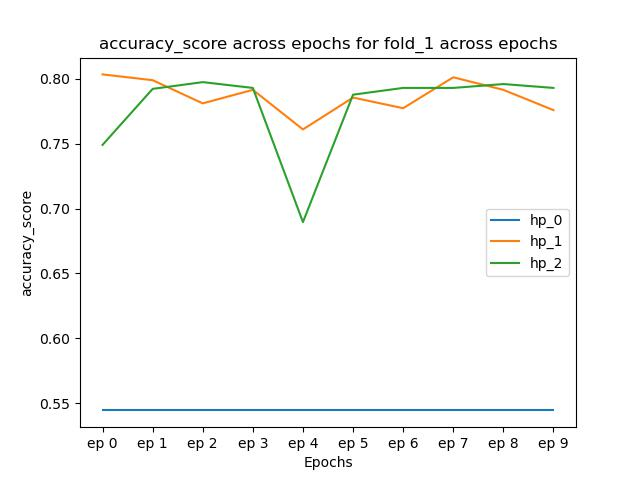
\includegraphics[scale = 0.75]{fold_1/accuracy_score}
\end{figure}
\subsection{f1\_score}
\begin{tabular}{lrrrrrrrrrr}
\toprule
{} &   ep 0 &   ep 1 &   ep 2 &   ep 3 &   ep 4 &   ep 5 &   ep 6 &   ep 7 &   ep 8 &   ep 9 \\
\midrule
hp\_0 &  0.705 &  0.705 &  0.705 &  0.705 &  0.705 &  0.705 &  0.705 &  0.705 &  0.705 &  0.705 \\
hp\_1 &  0.820 &  0.811 &  0.818 &  0.830 &  0.812 &  0.821 &  0.818 &  0.829 &  0.827 &  0.816 \\
hp\_2 &  0.788 &  0.821 &  0.827 &  0.824 &  0.775 &  0.815 &  0.815 &  0.817 &  0.818 &  0.814 \\
\bottomrule
\end{tabular}

\begin{figure}[H]
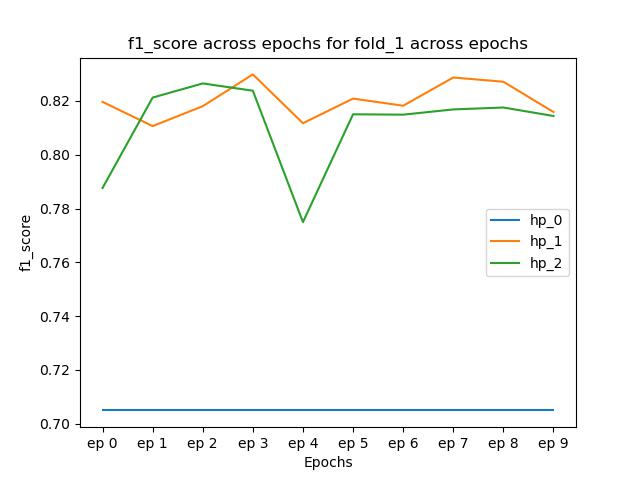
\includegraphics[scale = 0.75]{fold_1/f1_score}
\end{figure}
\subsection{precision\_score}
\begin{tabular}{lrrrrrrrrrr}
\toprule
{} &   ep 0 &   ep 1 &   ep 2 &   ep 3 &   ep 4 &   ep 5 &   ep 6 &   ep 7 &   ep 8 &   ep 9 \\
\midrule
hp\_0 &  0.544 &  0.544 &  0.544 &  0.544 &  0.544 &  0.544 &  0.544 &  0.544 &  0.544 &  0.544 \\
hp\_1 &  0.819 &  0.832 &  0.747 &  0.746 &  0.710 &  0.753 &  0.736 &  0.780 &  0.754 &  0.738 \\
hp\_2 &  0.730 &  0.772 &  0.774 &  0.767 &  0.640 &  0.775 &  0.794 &  0.788 &  0.796 &  0.795 \\
\bottomrule
\end{tabular}

\begin{figure}[H]
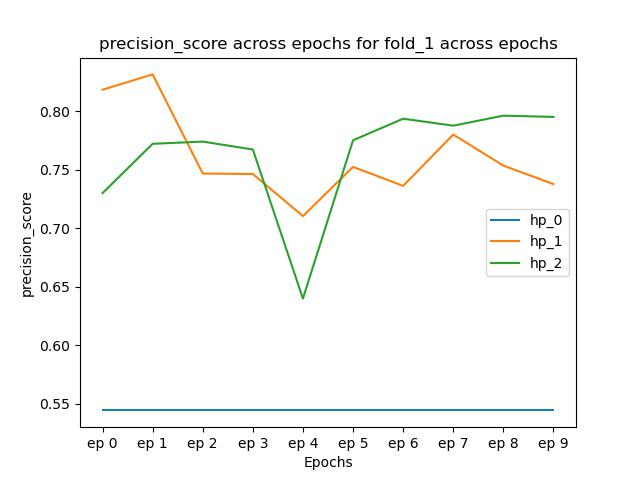
\includegraphics[scale = 0.75]{fold_1/precision_score}
\end{figure}
\subsection{matthews\_corrcoef}
\begin{tabular}{lrrrrrrrrrr}
\toprule
{} &   ep 0 &   ep 1 &   ep 2 &   ep 3 &   ep 4 &   ep 5 &   ep 6 &   ep 7 &   ep 8 &   ep 9 \\
\midrule
hp\_0 &  0.000 &  0.000 &  0.000 &  0.000 &  0.000 &  0.000 &  0.000 &  0.000 &  0.000 &  0.000 \\
hp\_1 &  0.604 &  0.598 &  0.565 &  0.593 &  0.542 &  0.574 &  0.563 &  0.601 &  0.588 &  0.558 \\
hp\_2 &  0.495 &  0.582 &  0.594 &  0.585 &  0.433 &  0.572 &  0.582 &  0.582 &  0.588 &  0.582 \\
\bottomrule
\end{tabular}

\begin{figure}[H]
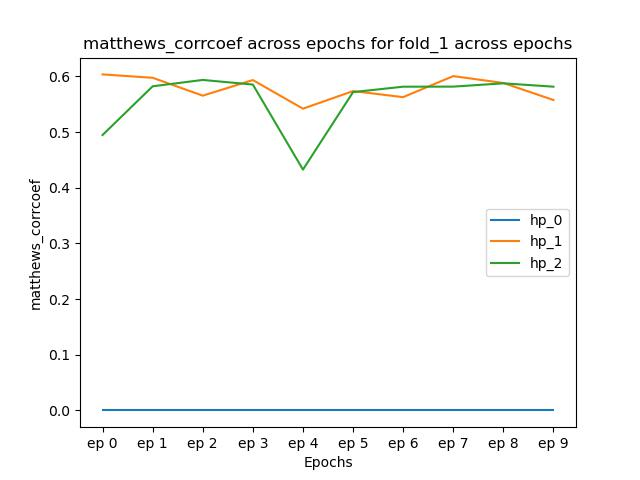
\includegraphics[scale = 0.75]{fold_1/matthews_corrcoef}
\end{figure}
\subsection{recall\_score}
\begin{tabular}{lrrrrrrrrrr}
\toprule
{} &   ep 0 &   ep 1 &   ep 2 &   ep 3 &   ep 4 &   ep 5 &   ep 6 &   ep 7 &   ep 8 &   ep 9 \\
\midrule
hp\_0 &  1.000 &  1.000 &  1.000 &  1.000 &  1.000 &  1.000 &  1.000 &  1.000 &  1.000 &  1.000 \\
hp\_1 &  0.821 &  0.791 &  0.904 &  0.934 &  0.947 &  0.903 &  0.921 &  0.884 &  0.917 &  0.912 \\
hp\_2 &  0.855 &  0.877 &  0.886 &  0.889 &  0.982 &  0.859 &  0.837 &  0.848 &  0.840 &  0.834 \\
\bottomrule
\end{tabular}

\begin{figure}[H]
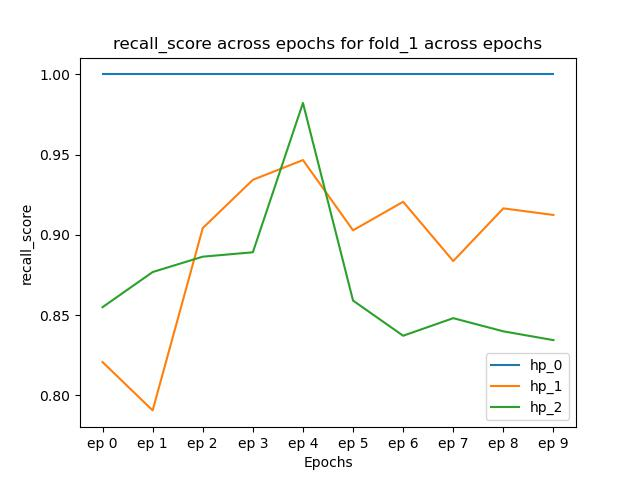
\includegraphics[scale = 0.75]{fold_1/recall_score}
\end{figure}
\end{document}
